\begin{figure}[t]
   \centering
   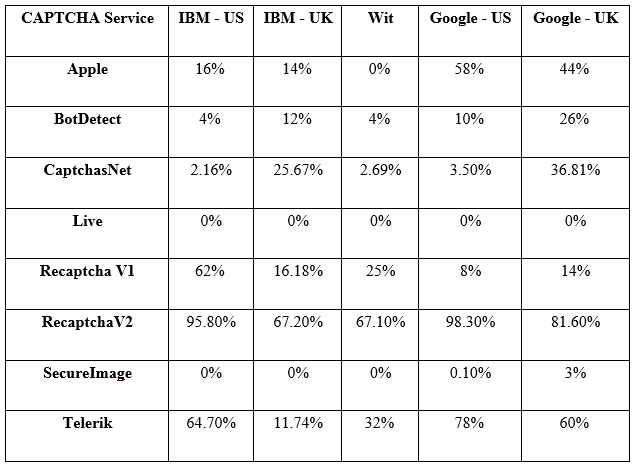
\includegraphics[width=\columnwidth]{figures/res1.png}.
   \caption{Results from our initial approach, before noise reduction.}
   \label{fig:results1}
\end{figure}


\section{Literature Review}
\label{sec:noisereduction}

This section gives a brief overview of what constitutes noise when it comes to human speech, a classification of the different kinds of noise and the audio processing techniques we used in our system to clean up the audio files.

\subsection{Sound}
Sound is created by alternate compression and decompression of particles of the air. This causes the air pressure to fall and rise in the form of waves. Frequency (pitch) and amplitude (loudness) are the two main characteristics of sound. \textbf{Frequency} is the number of times that the air is compressed and decompressed in a second, and is measured in cycles per second, or Hertz (Hz). Low frequency produces a low pitched, bass sound. High frequency produces a high pitched, whistle-like sound. Human ears respond to frequencies between 20Hz and 20,000Hz. \textbf{Amplitude} is the amount of sound energy reaching the eardrum, and is measured in decibels (dB). The safe range of amplitude for a human ear is 0 to 140dB.\newline

\subsection{Noise in Speech}
The human voice produces frequencies between 500Hz and 2,000Hz. Background noises have higher frequency levels than speech. The comprehension of speech is affected by both amplitude of the background noise and the amplitude of the voice itself. The average amplitude of a human voice in a room at a distance of one meter lies within the following ranges:
\begin{itemize}
\item Conversation	60-65dB
\item Dictation	65-70dB
\item Calling out	80-85dB 
\end{itemize}
The general background noise level must be at least 10dB lesser than these levels if the sound of the voice is to be heard clearly.\newline

\subsection{Classification of noise}
Noise can be broadly classified into 2 kinds - Internal noise and External noise.\newline

\textbf{Internal noise} is noise generated within the receiver or communication system. Colour noises like white noise, pink noise, brown noise,etc are examples of internal noises with specific characteristics, that can sometimes be manually added to mask other disrupting background noises. \textbf{External noise} is noise generated external to the system. So, all kinds of background noise come under this category.\newline

\subsection{Audacity}
We looked for a free, open-source, light-weight digital audio editing tool that was available in the market because our goal was to build a low-cost Audio CAPTCHA breaker. For this reason, we selected Audacity. Audacity is a free digital audio editor and recording tool that is available for Unix, Linux, OSX and Windows platforms. It has a number of built-in audio processing mechanisms that can be fine-tuned to our needs.\newline

\subsection{Audio processing techniques}
There are several audio processing techniques that are commonly used to remove noise and make recordings clearer in audio post-processing. All these techniques are available a single-click away in Audacity. So we exploit these functionalities without having to worry about the algorithm and the implementation. The following are some of the audio processing techniques that we use in this paper.\newline

\begin{itemize}
\item \textbf{Amplification} : Amplification is the process of increasing the amplitude of the audio by a certain amount or ratio. It just makes the audio sounding louder.
\item \textbf{Equalization} : Equalization is the process of adjusting the frequency response in an audio after recording. It is generally used to make certain sounds in an audio more prominent than others. We specifically use it to make vocal sounds louder and the background noises quieter.
\item \textbf{Normalization}: Normalization is done to set the peak amplitude of a track. A normalizer identifies the peak amplitude in the track and the maximum allowed amplitude and calculates gain as the difference between these two values. It then applies this gain for the entire track.
\item \textbf{Noise Gate} : Noise gates are used to remove constant background noises like hiss sounds, murmurs, leaf rustles, etc. It does this by allowing signals above a threshold amplitude value to pass through the gate, while blocking everything below.
\item \textbf{Noise Filter} : A noise filter is used to remove frequencies that do not fall within a certain range. To accomplish this, it uses 2 filters - a low pass filter that attenuates frequencies lower than  particular value and a high pass filter that attenuates frequencies higher than a particular value.
\item \textbf{Noise Reduction} : This technique samples a piece of the audio as a noise profile and applies a reduction in amplitude to the parts of the audio that has this noise.
\end{itemize}


